
\section*{Historical context}

\subsubsection{Scientific question}

Does the major-ion water chemistry in wetlands in the Western Cape Province show
geographical patterns?



\subsubsection{Computational context}

The research was done for a wetlands project \cite{Silberbauer:1991}, which 25 years later became the baseline for a project on changes in wetland status \cite{malan_trajectories_2015}. The project was managed by the Freshwater Research Unit (FRU), at that time a component of the University of Cape Town Zoology Department. In the 1980s, most �serious� computer work, especially statistics, was still done on a centralised mainframe using expensive packages such as BMDP and SPSS. Somewhere between 1986 and 1989 the FRU acquired a shared personal computer running Microsoft DOS, probably an AT with 1 Mb RAM and a 40 Mb hard drive, procured using external project funding, which budget records suggest cost about ZAR 15000 (similar to the prevailing value of a doctoral grant for one year). The IT equipment included an A3 dot-matrix graphics printer with a broad four-colour ribbon. Several staff members and students used the equipment under an analogue time-sharing system consisting of a paper calendar (see Appendix, Figure \ref{fig:fig_time}). 
\\Although I was familiar with mainframe Fortran 77 and IGL6 for graphics, Turbo Pascal seemed to me to be a more affordable PC compiler, with built-in graphics capability. A Turbo Pascal version 5 compiler cost ZAR 441.38, according to the hardcopy records in the project laboratory notebook (see Appendix, Figure \ref{fig:fig_cash}). The relational database was stored using PC-File, a Buttonware package based on the dBase format, and exported to a fixed-width text file for use by the Pascal Maucha program. To put the prices in context, a personal computer in 1986, with a staff discount, cost about ZAR 1800 (Bondwell IBM-PC AT clone with a Hercules graphics card and 20 Mb hard drive). 


Prof Jenny Day of the FRU advised the wetland team to use Maucha ionic diagrams \cite{maucha_hydrochemische_1932}, \cite{broch_modification_1969} for summarising the ratio of major cations and anions in water samples. She later used the software described here in a more extensive study of the dominance of major ions in South African rivers \cite{day_geographical_1995}. Constructing the diagrams, which were first used for visually classifying lake waters in Europe during the 1930s, is quite tedious, so preparing them with a computer program was a more cost-effective proposition.


Reproducibility and re-usability of code were not uppermost in my mind at that time � I needed to get the results out for project reports to the funding agency, and for publications. The original source code was never formally published, and funding for wetland research dried up at the end of 1989. I moved to a government remote sensing group with a VAX, running Fortran and C. Soon afterwards, the group adopted Esri�s Arc/Info as a graphics development platform on Sun Unix workstations, using the Arc Macro Language for programming. I could now code the symbols and mapping in a single program, and subsequent development followed a path of serial obsolescence: AML ? ArcView Avenue ? ArcGIS VBA. In 2010 I discovered that R could produce publishable maps of water quality distribution without the need for a licence server. The Maucha code now exists as a function in R.


\subsubsection{Retrieval of software}

The Pascal code was in the wetlands project directory in a forgotten corner of my computer�s hard drive - I copy everything over to the new drive when I upgrade my computer every few years. A copy of the code is available in the Appendix and in the Software Heritage Archive.

\section*{Dependencies}
The software has two dependencies, namely the Turbo Pascal compiler and a fixed-format ASCII file, CHEMDATA.DAT, containing the data. Both were still available in the project directory.

\section*{Execution}
Running 1980s software on a 2020s computer requires a virtual DOS environment. Fortunately, since the 1980s the Internet has happened, so I was able to find excellent instructions for running Turbo Pascal in DOSBox \cite{nevets_how_2016}, \cite{bartel_dosbox_2019}.


\begin{itemize}
    \item Hardware: Hewlett-Packard AMD Ryzen 7 PC
    \item Operating system: Windows 10 version 1903
    \item Turbo Pascal: version 5
\end{itemize}

No modification to the Pascal program was required. The directory in which the program
was located needed to be copied into a special DOSBox directory on the desktop.
The original instructions consisted of a few comment lines in the code.

The results obtained in the DOSBox virtual environment on a Windows 10 PC were similar to those in a 35mm slide presentation that I rediscovered in January 2020 \footnote{\href{https://photos.app.goo.gl/qqK6xKF46adjZDB37}{https://photos.app.goo.gl/qqK6xKF46adjZDB37}} (Figure \ref{fig:maucha_ab}). However, for the original publication, the process of preparing a figure would have comprised screen capture of the image, printing on paper and applying messy 20\textsuperscript{th} century analogue technology involving scissors and glue (Figure \ref{fig:fig_map}).


\begin{figure}[ht]
\begin{subfigure}{0.48\textwidth}
    \centering
    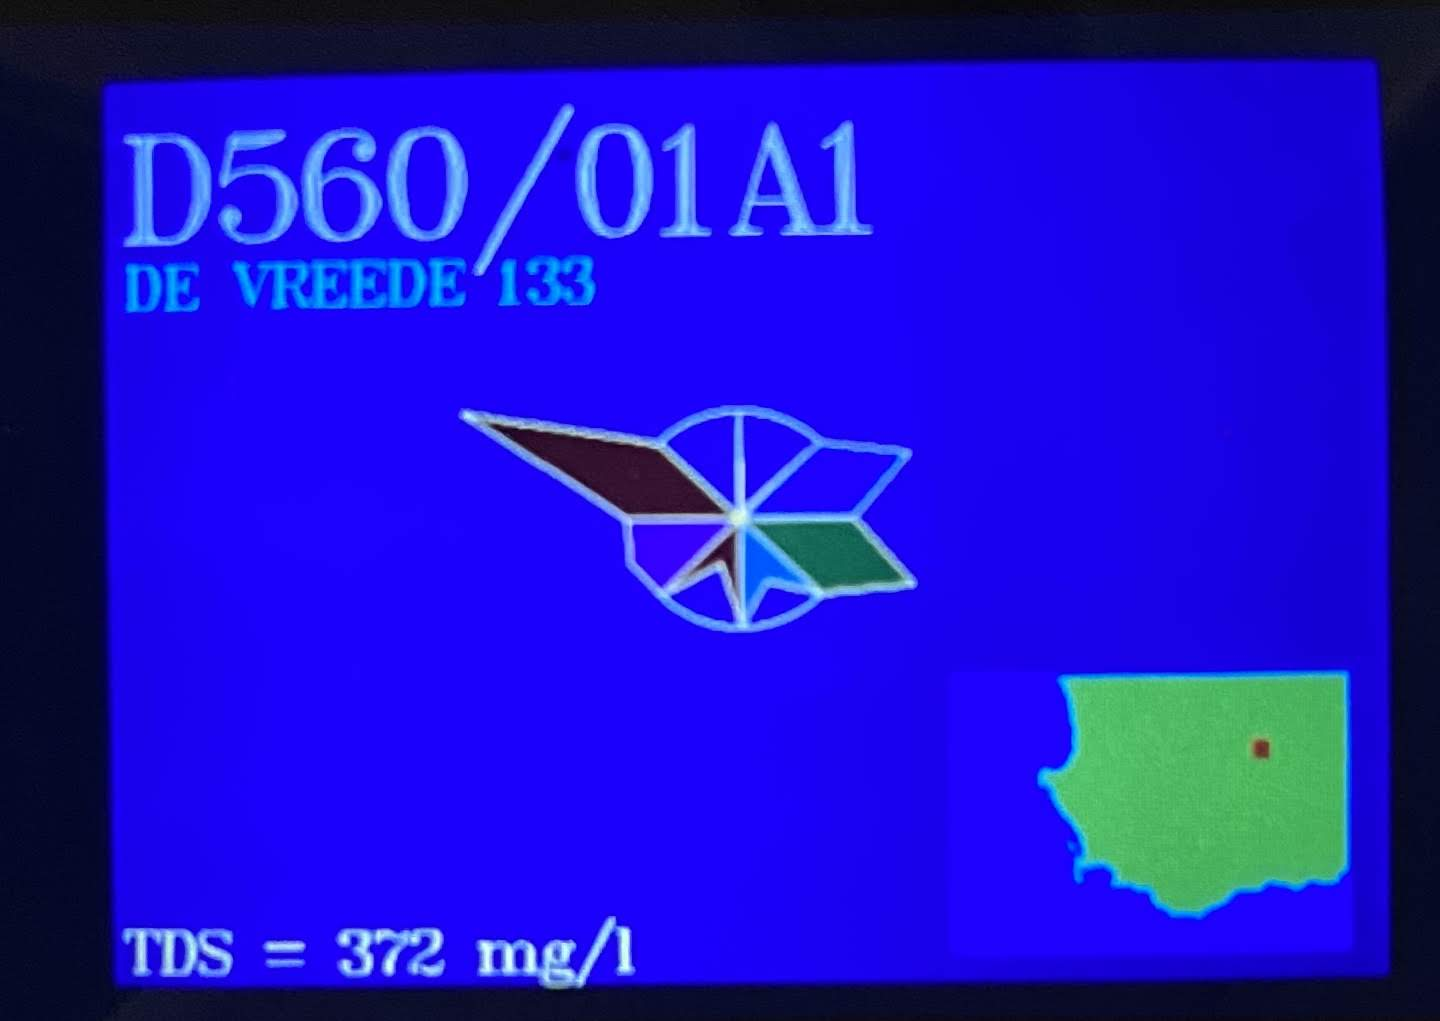
\includegraphics[height=4.6cm]{images/IMG_9611.jpg}
    \caption{}
    \label{fig:maucha_a}
\end{subfigure}
\begin{subfigure}{0.48\textwidth}
    \centering
    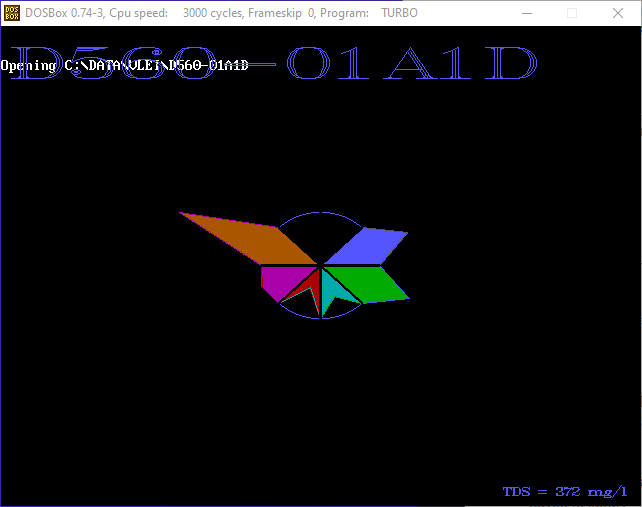
\includegraphics[height=4.6cm]{images/D560-01A1D.png}
    \caption{}
    \label{fig:maucha_b}
\end{subfigure}
\caption{Example of a Maucha diagram from a presentation dated 1989 (a) compared with a diagram generated using the Pascal program in DosBox during 2020 (b).}
\label{fig:maucha_ab}
\end{figure}


\begin{figure}[ht]
    \centering
    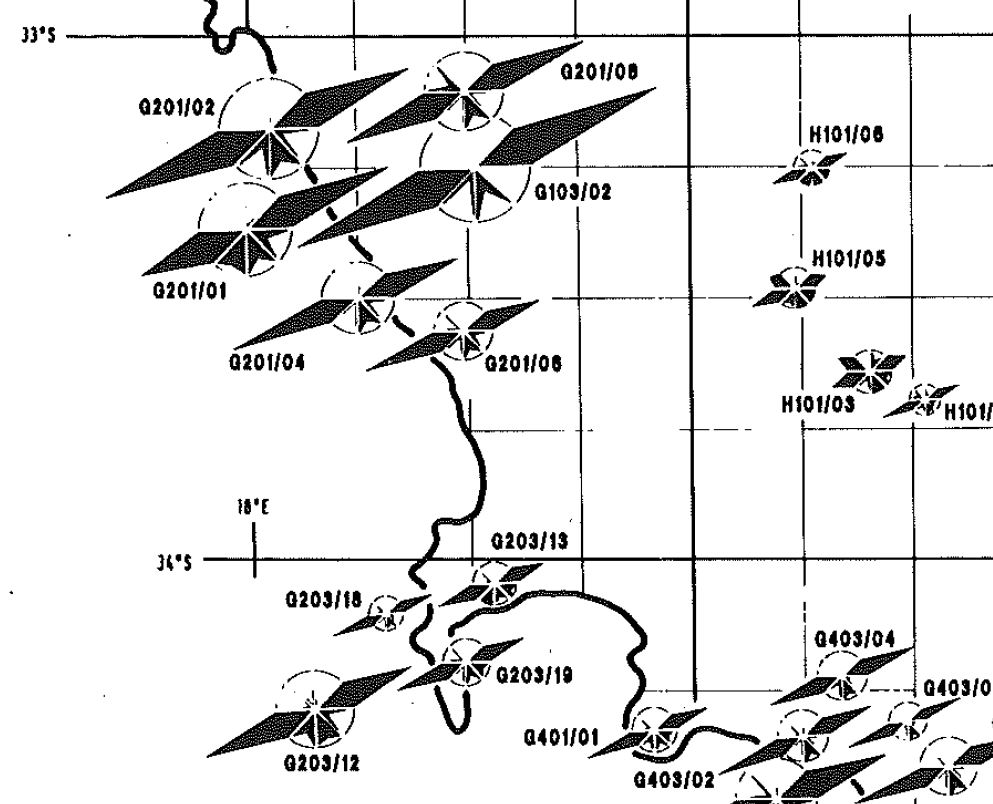
\includegraphics[width=0.95\linewidth]{images/SilberbauerKingFigure1.JPG}
    \caption{Map constructed in 1991 by printing screenshots of computer-generated Maucha symbols, cutting them out and gluing them to a background [1].}
    \label{fig:fig_map}
\end{figure}

\section*{Conclusion}
I would not advise anyone to use the original Turbo Pascal software. A recent R script \cite{silberbauer_internet-based_2020} or the Excel spreadsheet version\footnote{\href{http://www.riv.co.za/wv/Scripts.html}{http://www.riv.co.za/wv/Scripts.html}} would be easier to get going on a 21\textsuperscript{st} century computer. The competence that another researcher would need is knowledge of simple trigonometry and water chemistry. The original diagrams by Maucha in 1932 were drafted using paper and pencil, so in theory no programming skills are needed. In practice, constructing dozens of Maucha diagrams by hand, cutting them out and sticking them on a map, while initially therapeutic, could become impractical. On the occasion of my retirement in January 2020, a colleague kindly proved that the diagrams could also be produced in cake form  (Figure \ref{fig:fig_cake}). I regrettably cannot provide the code or recipe.
\\With regard to archiving software, this piece of code only survived in its original state because it was part of a project directory on my computer. More formal version control and archiving is recommended for important software.

\printbibliography
\clearpage
\appendix
\section*{Appendix}
\subsubsection{Source code}
Note that the constants hardcoded in \small{\texttt{procedure Equilivate}} are  atomic or molecular weights of each ion. 
\lstset{language=pascal}
\begin{lstlisting}

program MauchSpg;
{ Maucha R (1932) Hydrochemische Metoden in der Limnologie. Binnengewasser
    12, 173p.
  Broch E S & Yake W (1969) A modification of Maucha's ionic diagram
    to include ionic concentrations. Limnology & Oceanography 14 p 933-935 }
{ M J Silberbauer, Zoology University of Cape Town, September 1989 }
{ Modified to write to an Arc/Info Ungenerate file - MJS October 1992 }

{$R+} { check ranges }
Uses Graph;
var
   ChemFile   : Text;
   SpgFile    : Text;
   ChemValid  : boolean;
   Acidity    : boolean;
   SpgName    : string [64];
   VleiCode   : string [10];
   TextItem   : string [20];
   Pad        : string [1];
   X          : real;
   Y          : real;
   XAspect    : word;
   YAspect    : word;
   Aspect     : real;
   TotalArea  : real;
   IonArea    : real;
   TotalRadius: real;
   IonRadius  : real;
   XCentre    : integer;
   YCentre    : integer;
   SeedX      : integer;
   SeedY      : integer;
   XScreen    : integer;
   YScreen    : integer;
   I          : integer;
   Angle      : integer;
   Scale      : integer;
   StartAngle : real;
   IonAngle   : real;
   EndAngle   : real;
   Equivalents: real;
   EquivSum   : real;
   Vertex     : array[1..5,1..2] of integer;
   ChemInput  : array[1..9] of real;
   Gd, Gm     : integer;
   Temperature, Salinity, Conductivity, pH , TDS, TSS : real;
   CO3        , HCO3    , H2CO3       , Ca , Mg , Na  : real;
   K          , Cl      , S           , SO4, PO4      : real;
   SiO4       , TP      , KN          , NO3, NO2, NH4 : real;
   Polyphenol , WaterColour                           : real;
   Latitude   : real;
   Longitude  : real;

function r (Degree : real) : real;
begin
   r := Degree * Pi / 180;
end;

function ScaleX (XValue : real) : integer;      { scales x values }
begin
   XValue := XValue + (GetMaxX div 2);
   ScaleX := Round (XValue);
end;

function ScaleY (YValue : real) : integer;      { scales y values }
begin
   YValue := YValue * Aspect;
   YValue := YValue + (GetMaxY div 2);
   ScaleY := Round (YValue);
end;

procedure Equilivate;            { Converts mg/litre to meq/litre }
begin
   ChemInput[06] := CO3*2 / 50;  { "mg/l" originally obtained by multiplying}
   ChemInput[05] := HCO3  / 50;  {  meq/l by 50 (� mol. wt. of CaCO3)       }
   ChemInput[09] := H2CO3 / 50;
   ChemInput[01] := Ca*2  / 40.08;
   ChemInput[02] := Mg*2  / 24.31;
   ChemInput[08] := Na    / 22.99;
   ChemInput[07] := K     / 39.10;
   ChemInput[04] := Cl    / 35.45;
   ChemInput[03] := S*2   / 32.07;
end;


begin
   Assign (ChemFile, 'c:\data\vlei\CHEMDATA.DAT');
   Reset (ChemFile);
   Gd := Detect;
   InitGraph (Gd, Gm, '');
   if GraphResult <> grOK then Halt(1);
   SetTextStyle (TriplexFont, HorizDir, 1);
   SetTextJustify (LeftText, TopText);
   GetAspectRatio (XAspect, YAspect);
   Aspect := (XAspect / YAspect) * 0.9;

   Repeat
      For I := 1 to 9 do
      begin
         ChemInput[I] := -1;
      end;
      ReadLn (ChemFile, Latitude, Longitude, Latitude, Longitude,
              Temperature, Salinity, Conductivity, pH, TDS, TSS,
              CO3, HCO3, H2CO3, PO4, SiO4, TP, KN, NO3, NO2, NH4,
              Ca, Mg, Na, K, Cl, S,
              Polyphenol, WaterColour, Pad, Pad, VleiCode);
      Equilivate;

      ChemValid := true;
      EquivSum := 0;
      For I := 1 to 9 do
      begin
         If (ChemInput[I] < 0)  then ChemValid := false;
         EquivSum := EquivSum + ChemInput[I];
      end;

      Acidity := false;           { check for special case of acidity }
      if (H2CO3 > 0.01) then
      begin
         Acidity := true;
         ChemInput[05] := ChemInput[09]; { make bicarb represent acid.. }
      end;

      If (ChemValid) and (EquivSum > 0) then
      begin
         SpgName := Concat ('C:\DATA\VLEI\', VleiCode);
         WriteLn ('Opening ', SpgName);
         Assign (SpgFile, SpgName);
         Rewrite (SpgFile);

         XCentre     := 0;
         YCentre     := 0;
         TotalArea   := 4000 * Ln (EquivSum+1);
         TotalRadius := Sqrt (0.125 * TotalArea / Sin(r(22.5)));
         SetFillStyle (EmptyFill, 0);
         Ellipse     (ScaleX (XCentre), ScaleY (YCentre), 0, 360,
                      Round(TotalRadius), Round(TotalRadius * Aspect));

         FillEllipse (ScaleX (XCentre), ScaleY (YCentre),
                      Round(TotalRadius), Round(TotalRadius * Aspect));

         for Angle := 0 to 7 do
         begin
            Equivalents := ChemInput [Angle + 1];
            IonArea     := (Equivalents / EquivSum) * TotalArea;
            IonRadius   := IonArea / (TotalRadius * Sin(r(22.5)));
            StartAngle  := Angle * 45;
            IonAngle    := StartAngle + 22.5;
            EndAngle    := (Angle + 1) * 45;
            Vertex[1,1] := ScaleX (XCentre);
            Vertex[1,2] := ScaleY (YCentre);
            Vertex[2,1] := ScaleX (TotalRadius * Cos(r(StartAngle)));
            Vertex[2,2] := ScaleY (TotalRadius * Sin(r(StartAngle)));
            Vertex[3,1] := ScaleX (IonRadius   * Cos(r(IonAngle  )));
            Vertex[3,2] := ScaleY (IonRadius   * Sin(r(IonAngle  )));
            Vertex[4,1] := ScaleX (TotalRadius * Cos(r(EndAngle  )));
            Vertex[4,2] := ScaleY (TotalRadius * Sin(r(EndAngle  )));
            Vertex[5,1] := ScaleX (XCentre);
            Vertex[5,2] := ScaleY (YCentre);
            SeedX       := ScaleX (IonRadius/2.0 * Cos(r(IonAngle  )));
            SeedY       := ScaleY (IonRadius/2.0 * Sin(r(IonAngle  )));
            SetFillStyle (SolidFill, Angle+2);
            FillPoly (5, Vertex);
            SetColor (0);
            SetLineStyle (SolidLn, 0, ThickWidth);
                                      { Write to the Arc/Info Ungenerate file }
            WriteLn (SpgFile, Angle + 1, ',', SeedX, ',', SeedY);
            WriteLn (SpgFile, Vertex[1,1], ',', Vertex[1,2]);
            WriteLn (SpgFile, Vertex[2,1], ',', Vertex[2,2]);
            WriteLn (SpgFile, Vertex[3,1], ',', Vertex[3,2]);
            WriteLn (SpgFile, Vertex[4,1], ',', Vertex[4,2]);
            WriteLn (SpgFile, Vertex[5,1], ',', Vertex[5,2]);
            WriteLn (SpgFile, 'END');
            Line
            (Vertex[1,1], Vertex[1,2], Vertex[2,1], Vertex[2,2]);
            Line
            (Vertex[4,1], Vertex[4,2], Vertex[5,1], Vertex[5,2]);
            SetLineStyle (SolidLn, 0, NormWidth);
            SetColor (Angle+2);
         end;
         WriteLn (SpgFile, 'END');
         Close (SpgFile);
         X := TotalRadius * Sin(r(292.5));
         Y := TotalRadius * Cos(r(292.5));
         SetUserCharSize (2, 4, 2, 5);
         SetTextJustify (RightText, BottomText);
         Str (Round(TDS), TextItem);
         OutTextXY (GetMaxX-10, GetMaxY-10, 'TDS = ' + TextItem + ' mg/l');
         SetTextJustify (LeftText, BottomText);
         If (Acidity) then OutTextXY (20, GetMaxY-10, 'Acid');
         SetUserCharSize (3, 1, 3, 2);
         SetTextJustify (LeftText, TopText);
         OutTextXY (10,10,VleiCode);
         ReadLn;
         ClearDevice;
      end;
   until Eof (ChemFile);
   Close (ChemFile);
   SetUserCharSize (4, 3, 3, 3);
   EquivSum := 1;
   XCentre := 150;
   YCentre := 0;
   OutTextXY (XCentre + 40, YCentre, '[Equivalents]');
   SetTextJustify (LeftText, CenterText);
   for I := 1 to 5 do
   begin
      YCentre     := YCentre + 50;
      TotalArea   := 4000 * Ln (EquivSum+1);
      TotalRadius := Sqrt (0.125 * TotalArea / Sin(r(22.5)));
      Str (EquivSum:7:0, TextItem);
      OutTextXY (XCentre + Round(TotalRadius) + 10, YCentre, TextItem);
      SetFillStyle (EmptyFill, 0);
      Ellipse     (XCentre, YCentre, 0, 360,
                   Round(TotalRadius), Round(TotalRadius * Aspect));
      FillEllipse (XCentre, YCentre,
                   Round(TotalRadius), Round(TotalRadius * Aspect));
      EquivSum    := EquivSum * 10;
   end;
   ReadLn;
   CloseGraph;
end.
\end{lstlisting}

\subsection*{Examples of hardcopy records for the wetlands project}
The images in this section are a time sharing sheet for the only personal computer in the Freshwater Research Unit 
(Figure \ref{fig:fig_time}) and 
part of the analog spreadsheet of wetlands project expenditure
(Figure \ref{fig:fig_cash}).
The final figure is a nutritious data reporting format produced three decades later
(Figure \ref{fig:fig_cake}).

\begin{figure}[ht]
    \centering
    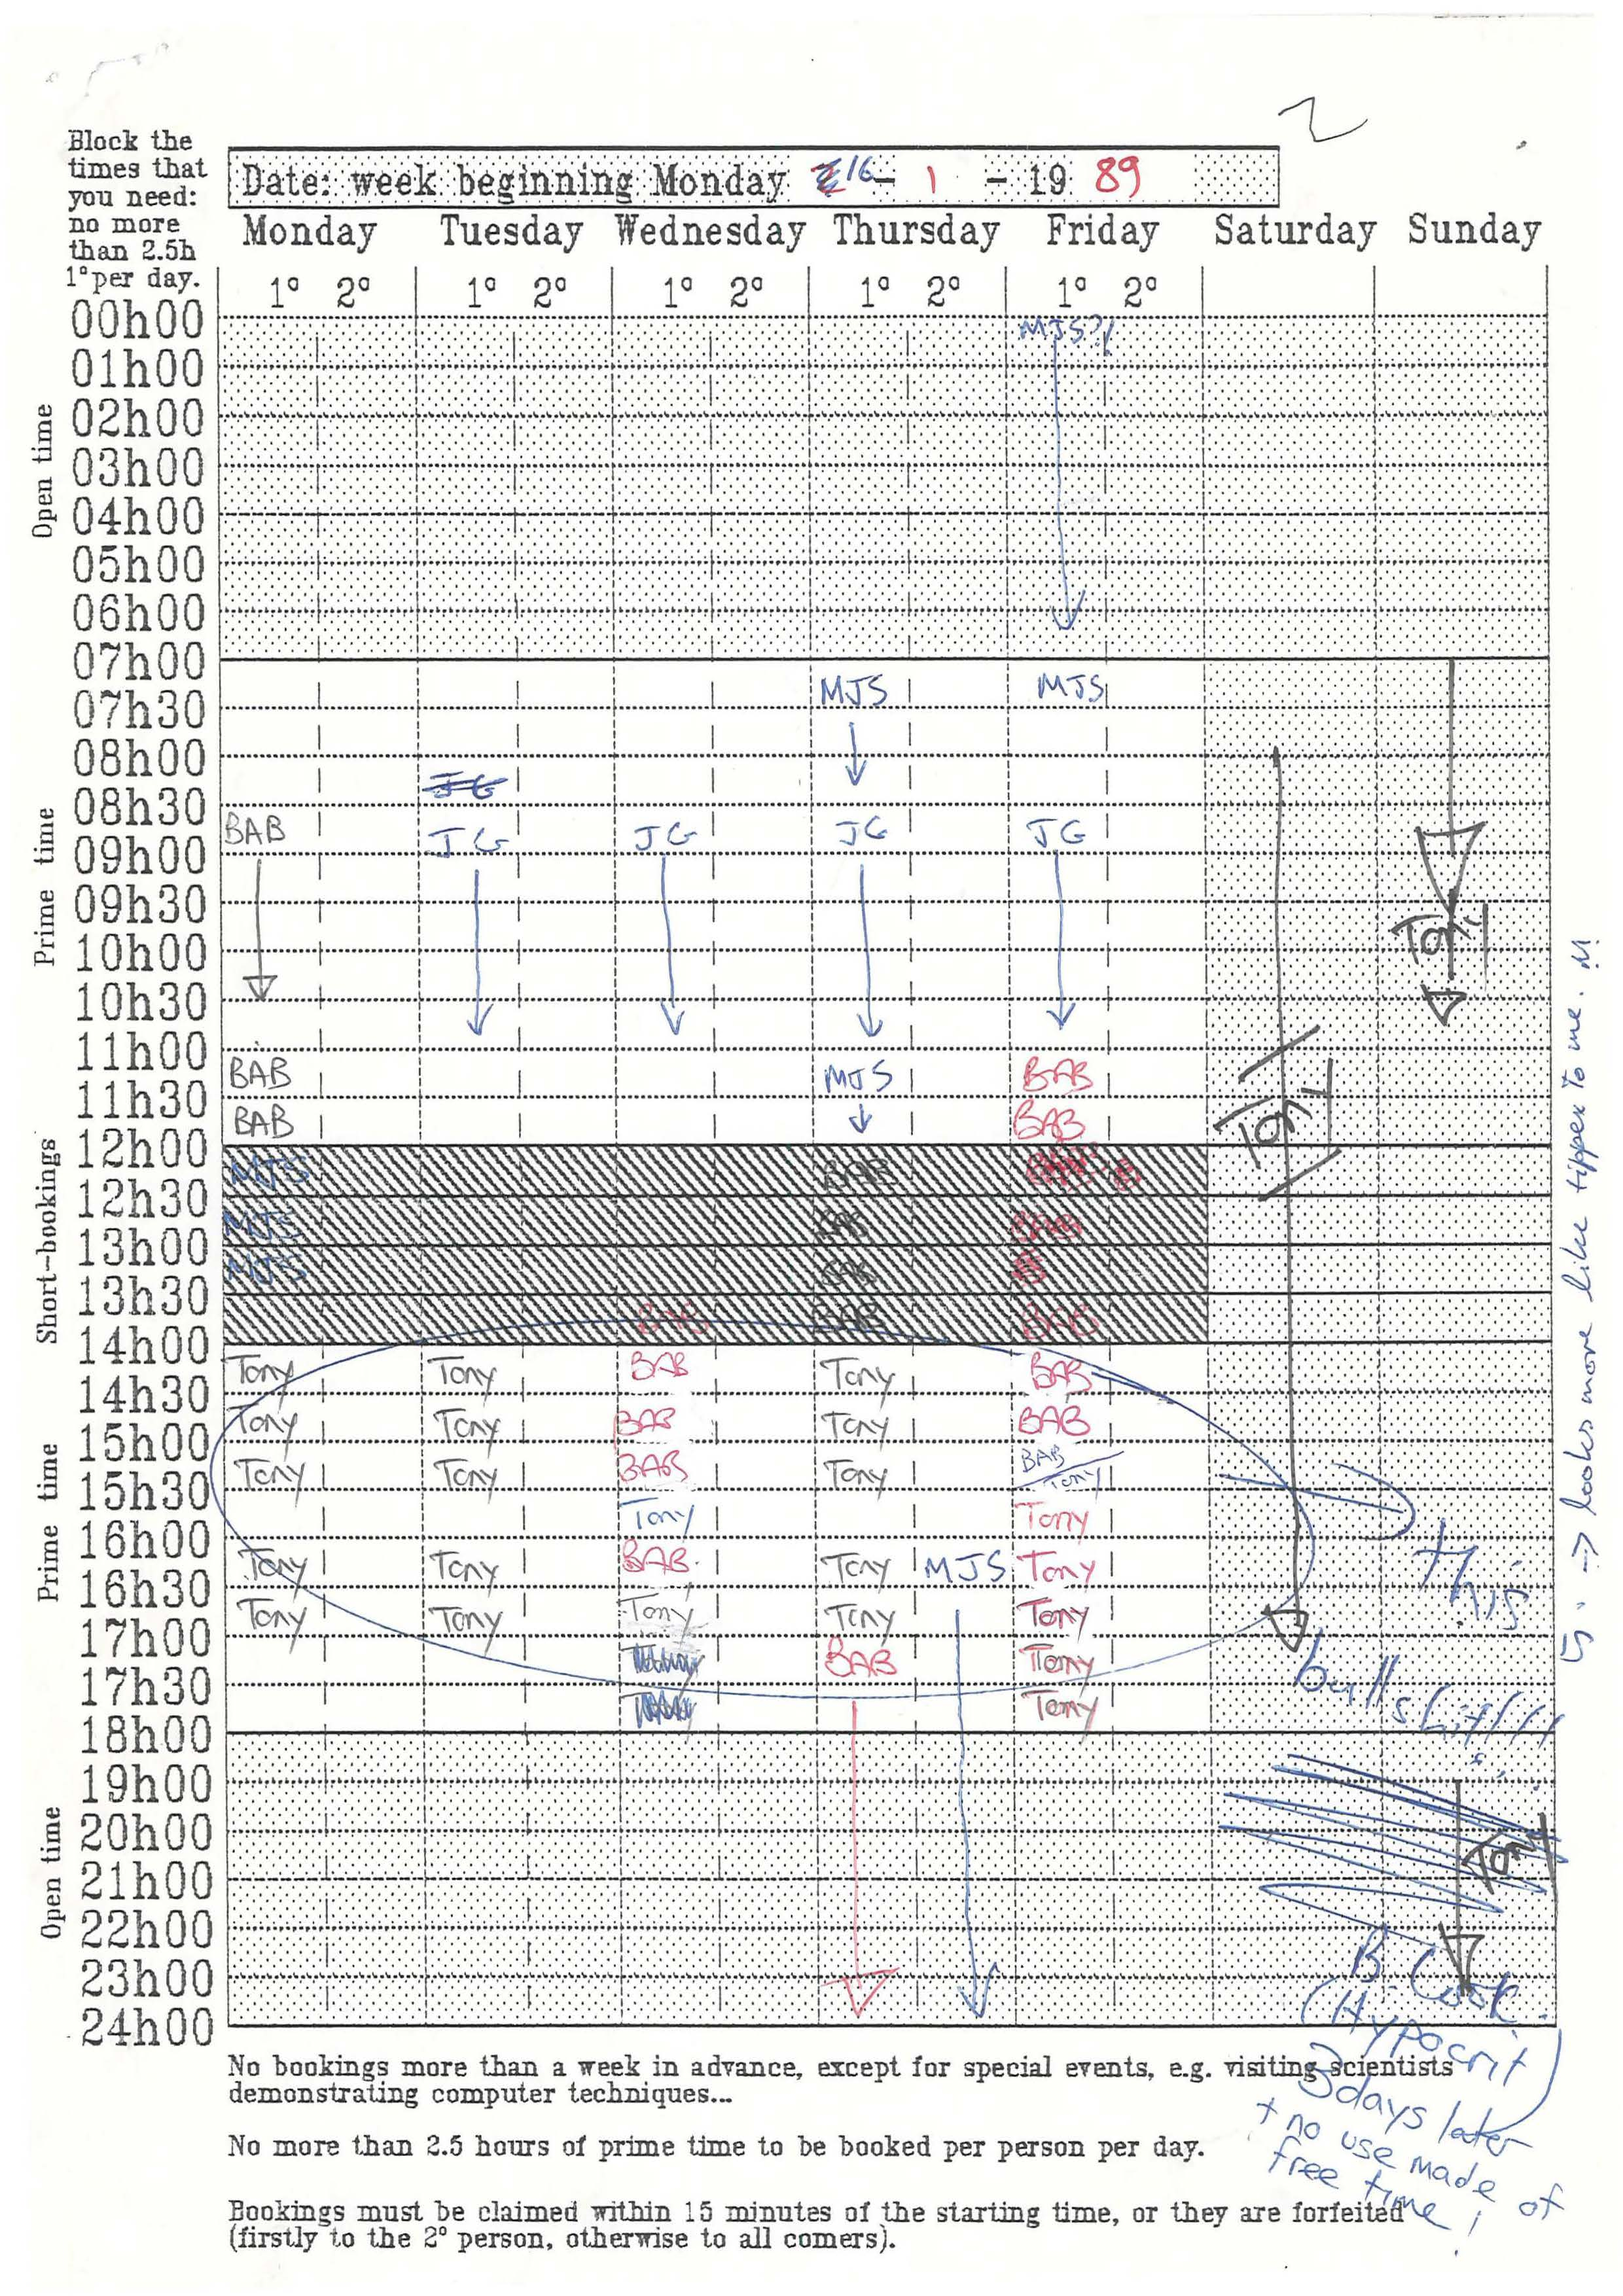
\includegraphics[width=0.85\linewidth]{images/FRU_1989_PC_booking_Page_03.jpg}
    \caption{Example of time-sharing sheet for the FRU computer in 1989. Observe how flame wars originated before Internet social media.}
    \label{fig:fig_time}
\end{figure}


\begin{figure}[ht]
    \centering
    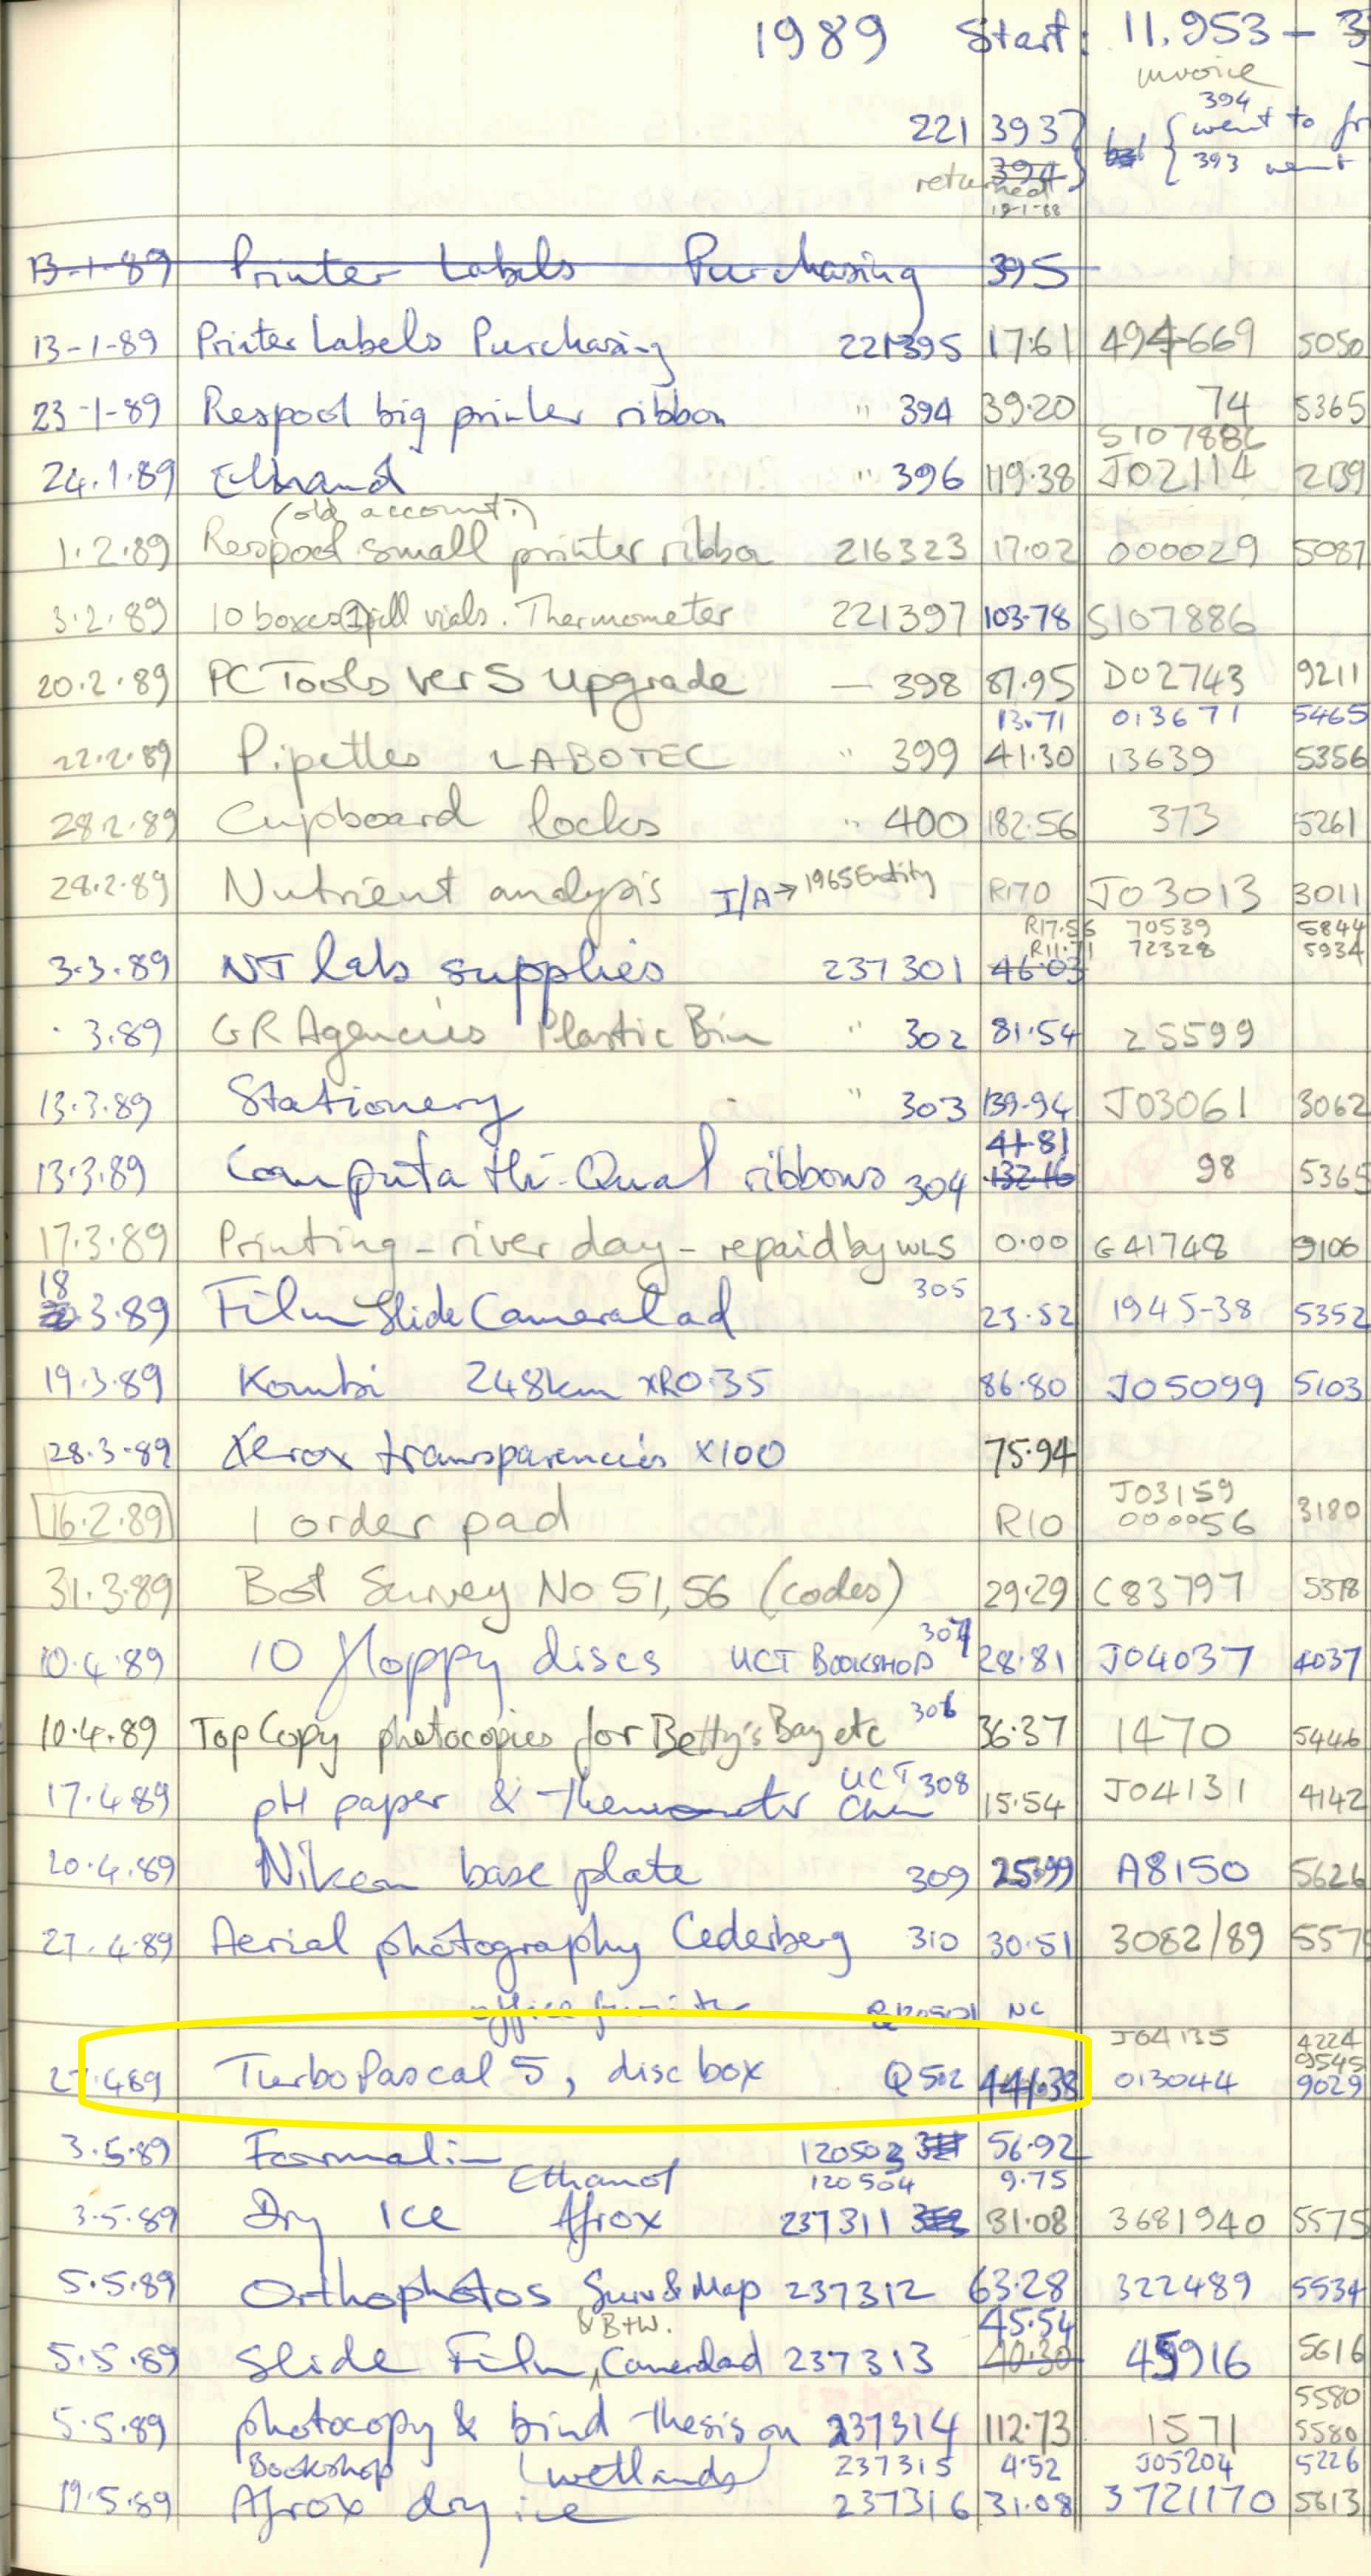
\includegraphics[width=0.85\linewidth]{images/Price_TurboPascal_4_1989.jpg}
    \caption{Record of project purchases in 1989.}
    \label{fig:fig_cash}
\end{figure}


\begin{figure}[ht]
    \centering
    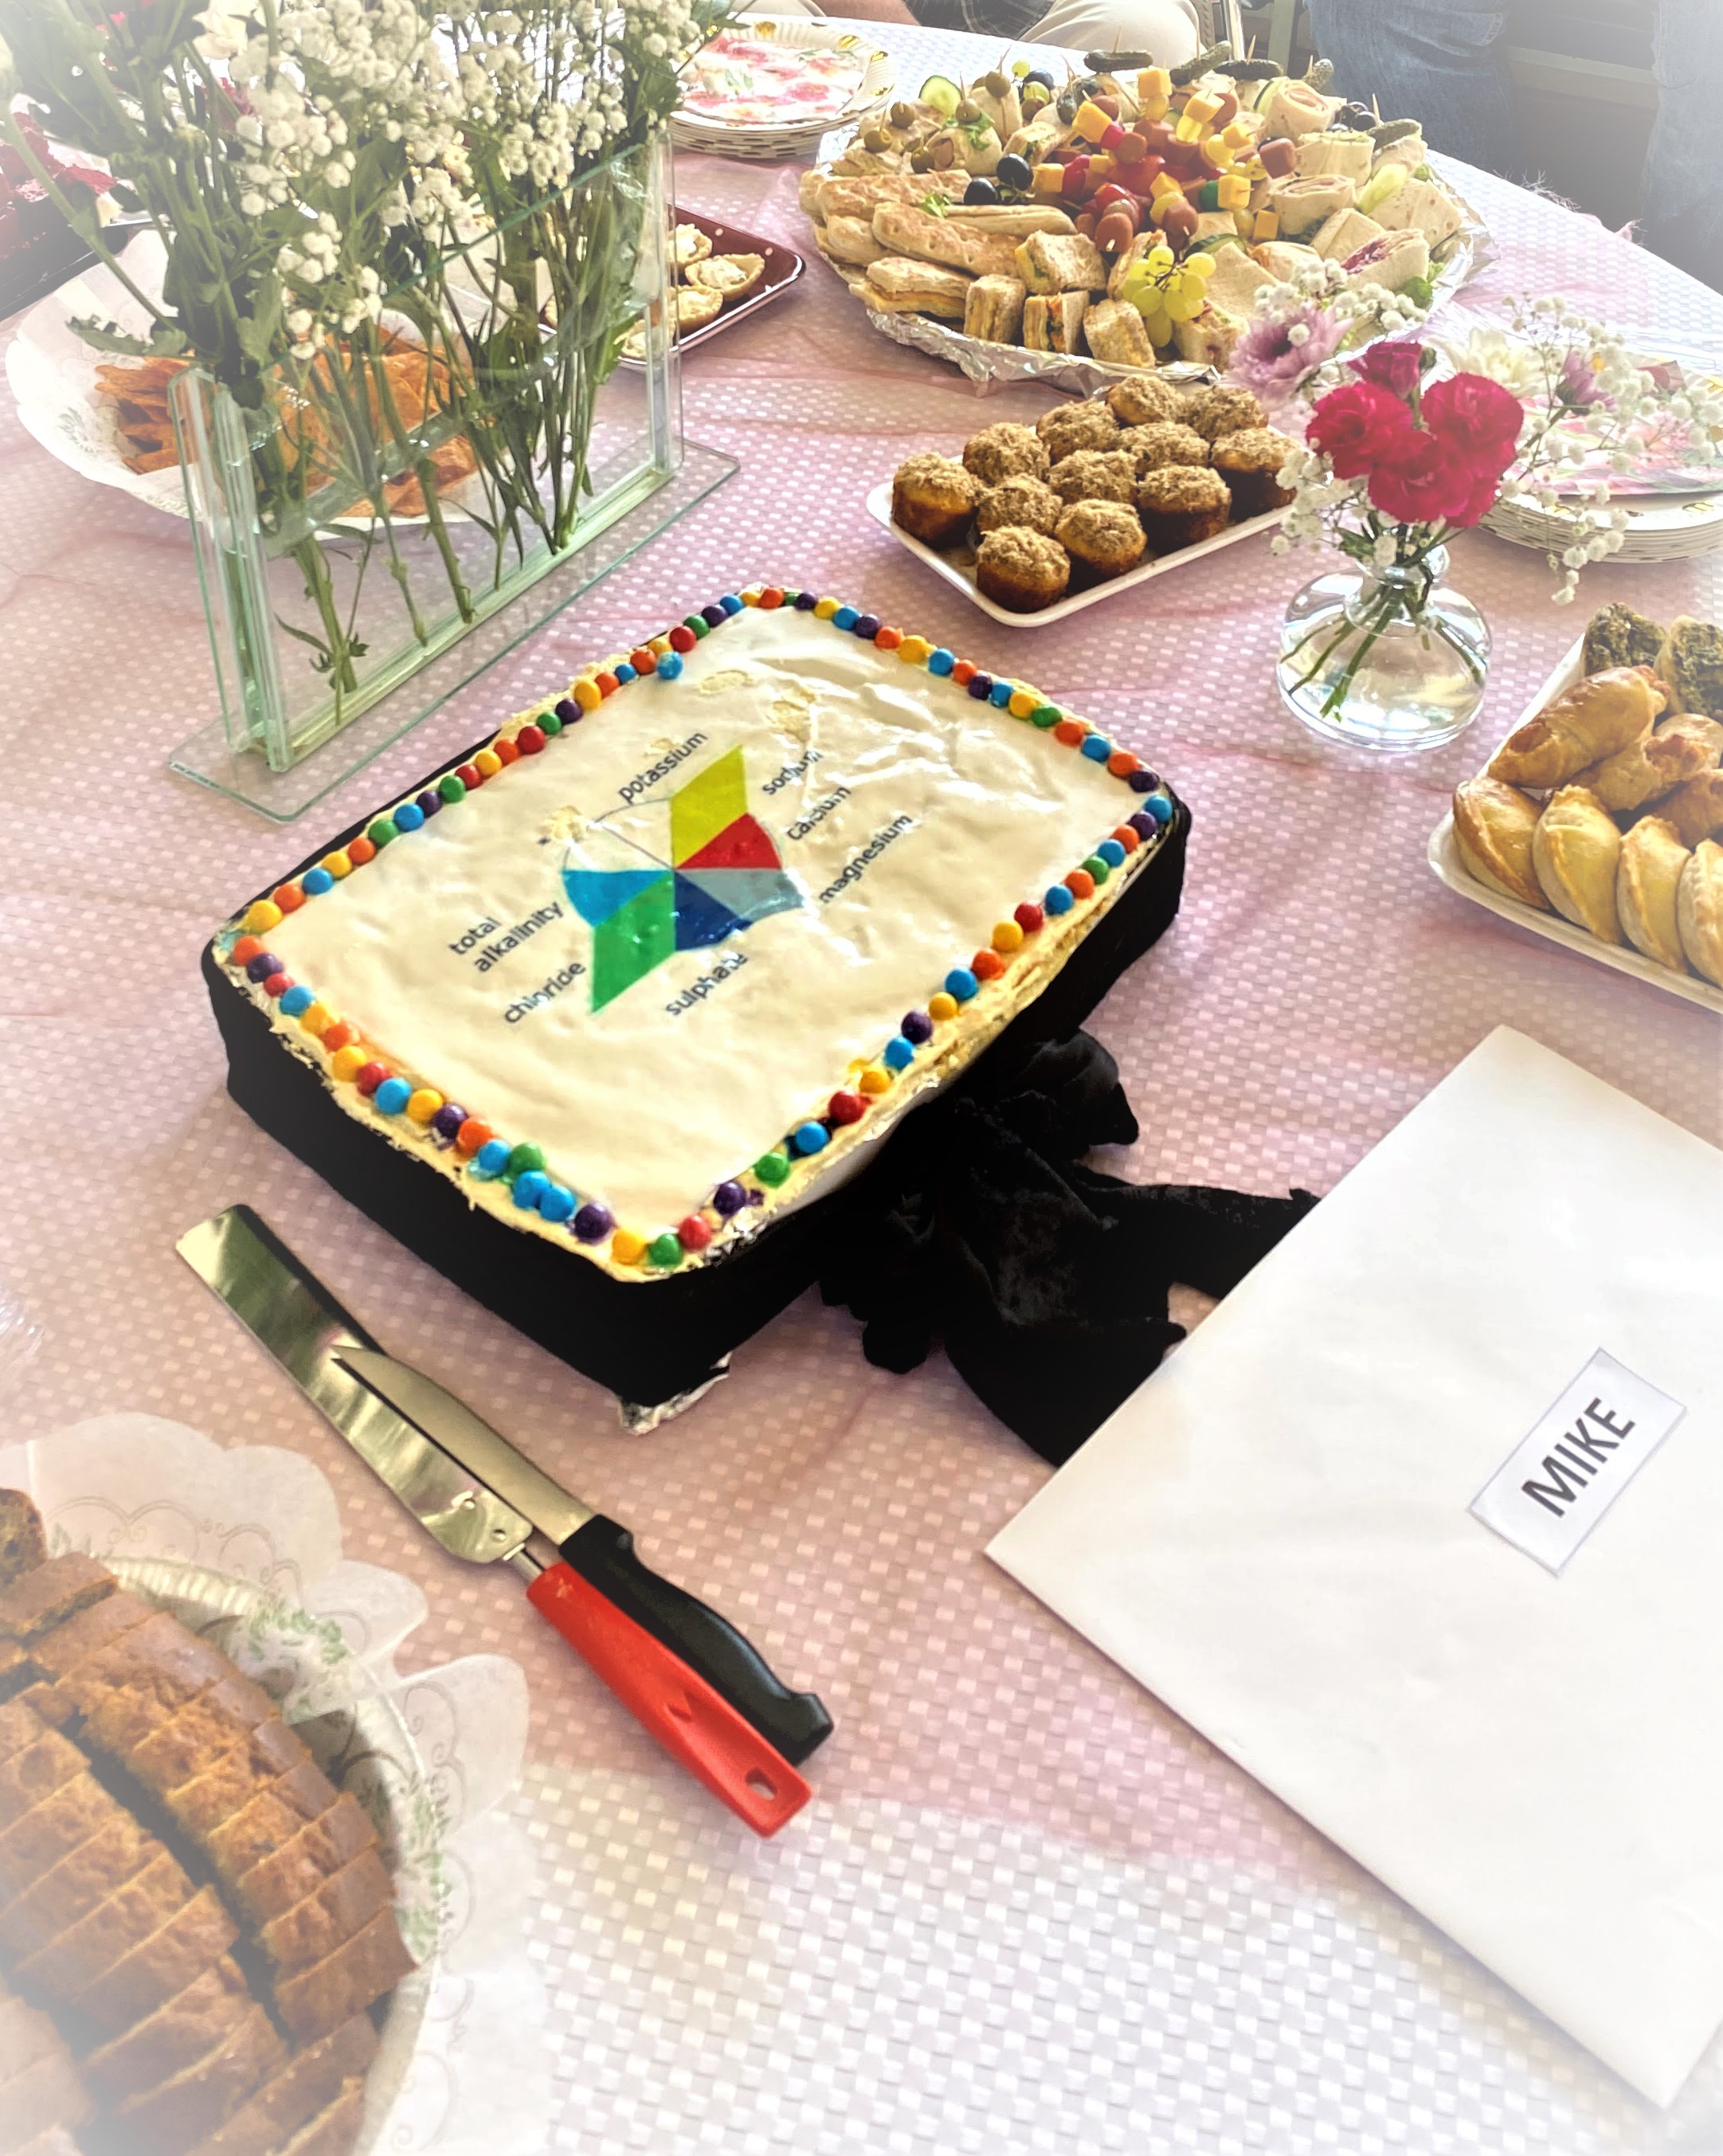
\includegraphics[width=0.85\linewidth]{images/Maucha_Cake_2020-01-31.jpg}
    \caption{Example of Maucha ionic diagram in cake format, by M Cilliers, University of Pretoria.}
    \label{fig:fig_cake}
\end{figure}
